%%%%%%%%%%%%%%%%%%%%%%%%%%%%%%%%%%%%%%%%%
% FRI Data Science_report LaTeX Template
% Version 1.0 (28/1/2020)
% 
% Jure Demšar (jure.demsar@fri.uni-lj.si)
%
% Based on MicromouseSymp article template by:
% Mathias Legrand (legrand.mathias@gmail.com) 
% With extensive modifications by:
% Antonio Valente (antonio.luis.valente@gmail.com)
%
% License:
% CC BY-NC-SA 3.0 (http://creativecommons.org/licenses/by-nc-sa/3.0/)
%
%%%%%%%%%%%%%%%%%%%%%%%%%%%%%%%%%%%%%%%%%


%----------------------------------------------------------------------------------------
%	PACKAGES AND OTHER DOCUMENT CONFIGURATIONS
%----------------------------------------------------------------------------------------
\documentclass[fleqn,moreauthors,10pt]{ds_report}
\usepackage[english]{babel}

\graphicspath{{fig/}}




%----------------------------------------------------------------------------------------
%	ARTICLE INFORMATION
%----------------------------------------------------------------------------------------

% Header
\JournalInfo{FRI Natural language processing course 2021}

% Interim or final report
\Archive{Project report} 
%\Archive{Final report} 

% Article title
\PaperTitle{Unsupervised Domain adaptation for Sentence Classification} 

% Authors (student competitors) and their info
\Authors{Marko Možina, Peter Kosem, Aljaž Konec}

% Advisors
\affiliation{\textit{Advisors: Boshko Koloski}}

% Keywords
\Keywords{Unsupervised Sentence Classification, Generative Pseudo Labeling, Transformer-based Denoising AutoEncoder}
\newcommand{\keywordname}{Keywords}


%----------------------------------------------------------------------------------------
%	ABSTRACT
%----------------------------------------------------------------------------------------

\Abstract{
TBA
}

%----------------------------------------------------------------------------------------

\begin{document}

% Makes all text pages the same height
\flushbottom 

% Print the title and abstract box
\maketitle 

% Removes page numbering from the first page
\thispagestyle{empty} 

%----------------------------------------------------------------------------------------
%	ARTICLE CONTENTS
%----------------------------------------------------------------------------------------

\section*{Introduction}

Natural Language Processing (NLP) significantly benefits applications like sentiment analysis, spam detection, and topic categorization. The challenge intensifies when applying general NLP models to specialized domains, where unique terminologies and contexts can affect model performance. Sentence-transformer models, while effective for generating sentence embeddings, often fall short in these specialized settings without domain-specific tuning.

This project aims to tackle this issue by enhancing sentence representation in specialized domains through unsupervised domain adaptation techniques, specifically Transformer-based Denoising AutoEncoder (TSDAE) and Generative Pse\-udo Labeling (GPL). These methods intend to refine the embedding space, making models more sensitive and accurate for specific domains, thereby improving sentence classification outcomes.

By investigating the application of TSDAE and GPL for domain adaptation, this study seeks to bridge the gap between general-purpose sentence embeddings and their effectiveness in domain-specific contexts, offering potential improvements in NLP model performance across specialized fields.


%------------------------------------------------

\section*{Methods}

This section outlines the approach taken to adapt sentence-transformer models for improved sentence classification within specialized domains, leveraging the techniques of Transformer-based Denoising AutoEncoder (TSDAE) and Generative Pse\-udo Labeling (GPL).

\subsection*{Generative pseudo labeling (GPL)}

In the vast landscape of digital information, the ability to effectively process and classify text across diverse domains remains a paramount challenge in natural language processing. Traditional models often falter when applied outside their training domain due to the unique linguistic characteristics of new data sets. This gap highlights the urgent need for domain adaptation techniques capable of leveraging the wealth of unlabeled textual data prevalent in specialized fields. Generative Pseudo Labeling (GPL) emerges as a vital solution, offering a novel approach to utilize unlabeled data for enhancing model adaptability and performance in uncharted domains.

Generative Pseudo Labeling (GPL) is predicated on the innovative use of unlabeled data to improve model functionality in target domains. The GPL methodology unfolds in two pivotal stages:
\begin{enumerate}
    \item \textbf{Pseudo Label Generation:} A pre-trained model, proficient in a related but distinct task, assigns provisional labels to unlabeled target domain data. These initial labels, derived from the model's pre-existing knowledge, serve as a foundational step for domain adaptation ~\cite{reimers2019sentence}.
    
    \item \textbf{Refinement through Generative Modeling:} Subsequently, the model undergoes a self-enhancement phase, refining its capabilities by learning from the data directly. This involves generative models that discern and adapt to the underlying patterns specific to the target domain, thereby aligning the model more closely with the target domain's characteristics ~\cite{wang-etal-2022-gpl}.
\end{enumerate}

Our project seeks to leverage GPL for the unsupervised domain adaptation of sentence-transformer models, aiming to bolster sentence classification accuracy within specialized domains. The application process is outlined as follows:
\begin{enumerate}
    \item \textbf{Initial Model Training:} Employing a pre-trained sent\-ence-transformer model, leveraging its extensive knowledge base for a preliminary understanding of the target domain ~\cite{reimers2019sentence}.
    
    \item \textbf{Pseudo Label Creation:} Generating pseudo labels for the Slovenian classification dataset (e.g., SentiNews) with the pre-trained model, bridging the model's knowledge from general to specific domains.

    \item \textbf{Model Adaptation via GPL:} A generative model refines the sentence embeddings and classification efficacy of the sentence-transformer, emphasizing the adaptation to capture domain-specific nuances accurately ~\cite{wang-etal-2022-gpl}.

    \item \textbf{Iterative Refinement and Evaluation:} Through continuous refinement and evaluation, the model's performance is iteratively improved, ensuring its alignment with the project's goals.
\end{enumerate}



\subsection*{Transformer-based Denoising AutoEncoder (TSDAE)}

The core idea of TSDAE is to introduce noise to input sequences by deleting or swapping tokens (e.g., words). This corrupted input is then fed into the encoder component of the TSDAE, which consists of transformer layers that encode the corrupted input data into a latent space representation of sentence vectors. Decoder network, which also consists of transformer layers, then aims to reconstruct the original, clean input data from the latent representation. Below, we briefly explain the sequential process of TSDAE:

\begin{enumerate}
    \item \textbf{Corruption:} The input data is corrupted with noise, introducing variations and disturbances into the data. Adopting only deletion as the input noise and setting the deletion ratio to 0.6 performs best per~\cite{wang2021tsdae}.
    \item \textbf{Encoding:} The corrupted input data is fed into the encoder, which consists of transformer layers. These layers transform the input data into a latent space representation called sentence vector, capturing essential features while filtering out noise.
    \item \textbf{Decoding:} The latent representation obtained from the encoder is passed through the decoder, also composed of Transformer layers. The decoder aims to reconstruct the original, clean input data from the latent representation.
    \item \textbf{Reconstruction:} The classifier token (CSL) embedding is used during reconstruction from token-level to sentence-level representation~\cite{pinecone_2021}.
    \item \textbf{Training:} The TSDAE optimizes its parameters by minimizing the reconstruction error between the denoised output generated by the decoder and the original, clean input data. This process occurs iteratively, allowing the model to learn effective denoising strategies.
\end{enumerate}

For fine-tuning the model, we need to set up the training data (which is nothing more than text data, since the model is unsupervised), a pretrained model prepared for producing sentence vectors and a loss function.

By leveraging the Transformer architecture, TSDAEs can efficiently capture complex dependencies and patterns in the data, making them effective for denoising tasks across various domains, including natural language processing. Despite its inability to match the performance of supervised methods, TSDAE remains valuable, particularly in scenarios where data is unlabeled or difficult to obtain.

\section*{initial Evaluation of TSDAE Models}

\subsection*{Objective}

This section presents the initial experimental evaluation of various sentence-transformer models, specifically focusing on their performance in sentence classification tasks within the context of unsupervised domain adaptation. The primary objective was to compare the effectiveness of traditional transformer models against their TSDAE-adapted counterparts.



\subsection*{Experimental Setup}

The experiments were conducted using three different models: ``bert-base-multilingual-uncased'', ``all-MiniLM-L12-v2'', and ``hate\_speech\_slo''. Each model was evaluated in its base configuration as well as its TSDAE-modified version. The models were trained on a subset of 10,000 sentences extracted from the SentiNews dataset, aiming to establish preliminary performance metrics.

The dataset was split into training and testing sets with an 80-20 ratio, using a random seed for reproducibility. Model training was followed by sentence embedding generation for both training and testing datasets. Logistic regression was then applied to these embeddings to perform sentence classification, assessing the models based on their F1 scores and log loss metrics.

\subsection*{Results}
The performance of each model is summarized as follows:

\begin{itemize}
    \item \textbf{BERT Base Multilingual Uncased}: Achieved an F1 score of 0.606 and a log loss of 0.756. Its TSDAE variant recorded a slightly lower F1 score of 0.604 and a higher log loss of 0.764.
    \item \textbf{Hate Speech SLO}: Mirrored the BERT base model in F1 score (0.606) and log loss (0.756), while its TSDAE adaptation saw a decrease in performance with an F1 score of 0.602 and a log loss of 0.774.
    \item \textbf{All-MiniLM-L12-v2}: The base model had an F1 score of 0.561 and a log loss of 0.820, with the TSDAE adaptation further decreasing in F1 to 0.541 and increasing log loss to 0.826.
\end{itemize}

The following table illustrates these results in detail:

\begin{table}[h]
\centering
\begin{tabular}{|l|c|c|}
\hline
\textbf{Model} & \textbf{F1 Score} & \textbf{Log Loss} \\
\hline
bert-base-multiling.-uncased & 0.606 & 0.756 \\
tsdae-bert-base-multiling.-uncased & 0.604 & 0.764 \\
hate\_speech\_slo & 0.606 & 0.756 \\
tsdae-hate\_speech\_slo & 0.602 & 0.774 \\
all-MiniLM-L12-v2 & 0.561 & 0.820 \\
tsdae-all-MiniLM-L12-v2 & 0.541 & 0.826 \\
\hline
\end{tabular}
\caption{Performance metrics of base and TSDAE models.}
\label{table:tsdae_performance}
\end{table}

\subsection*{Analysis}

The results indicate a slight performance decrease for TSDAE models compared to their base counterparts across the models tested. This could be attributed to several factors, including the complexity of the domain adaptation task, the characteristics of the dataset, and the inherent challenges in using unsupervised methods for domain-specific sentence classification. Additionally, the TSDAE models were only trained on 10,000 sentences, which may have contributed to their relatively poorer performance due to insufficient training data. Furthermore, the increase in log loss suggests that while TSDAE models may be refining the sentence embeddings, they might also be introducing aspects that do not correlate as effectively with the classification objectives as the original models.


\subsection*{Future Work}

Further investigations will focus on optimizing the TSDAE training process, exploring different configurations of noise and corruption techniques, and increasing the dataset size to improve the robustness and accuracy of the models. Additionally, deeper analysis into the types of errors made by the TSDAE models may provide insights into their operational dynamics and potential areas for enhancement.


% You can write equations inline, e.g. $\cos\pi=-1$, $E = m \cdot c^2$ and $\alpha$, or you can include them as separate objects. The Bayes’s rule is stated mathematically as:

% \begin{equation}
% 	P(A|B) = \frac{P(B|A)P(A)}{P(B)},
% 	\label{eq:bayes}
% \end{equation}

% where $A$ and $B$ are some events. You can also reference it -- the equation \ref{eq:bayes} describes the Bayes's rule.

% \subsection*{Lists}

% We can insert numbered and bullet lists:

% % the [noitemsep] option makes the list more compact
% \begin{enumerate}[noitemsep] 
% 	\item First item in the list.
% 	\item Second item in the list.
% 	\item Third item in the list.
% \end{enumerate}

% \begin{itemize}[noitemsep] 
% 	\item First item in the list.
% 	\item Second item in the list.
% 	\item Third item in the list.
% \end{itemize}

% We can use the description environment to define or describe key terms and phrases.

% \begin{description}
% 	\item[Word] What is a word?.
% 	\item[Concept] What is a concept?
% 	\item[Idea] What is an idea?
% \end{description}


% \subsection*{Random text}

% This text is inserted only to make this template look more like a proper report. Lorem ipsum dolor sit amet, consectetur adipiscing elit. Etiam blandit dictum facilisis. Lorem ipsum dolor sit amet, consectetur adipiscing elit. Interdum et malesuada fames ac ante ipsum primis in faucibus. Etiam convallis tellus velit, quis ornare ipsum aliquam id. Maecenas tempus mauris sit amet libero elementum eleifend. Nulla nunc orci, consectetur non consequat ac, consequat non nisl. Aenean vitae dui nec ex fringilla malesuada. Proin elit libero, faucibus eget neque quis, condimentum laoreet urna. Etiam at nunc quis felis pulvinar dignissim. Phasellus turpis turpis, vestibulum eget imperdiet in, molestie eget neque. Curabitur quis ante sed nunc varius dictum non quis nisl. Donec nec lobortis velit. Ut cursus, libero efficitur dictum imperdiet, odio mi fermentum dui, id vulputate metus velit sit amet risus. Nulla vel volutpat elit. Mauris ex erat, pulvinar ac accumsan sit amet, ultrices sit amet turpis.

% Phasellus in ligula nunc. Vivamus sem lorem, malesuada sed pretium quis, varius convallis lectus. Quisque in risus nec lectus lobortis gravida non a sem. Quisque et vestibulum sem, vel mollis dolor. Nullam ante ex, scelerisque ac efficitur vel, rhoncus quis lectus. Pellentesque scelerisque efficitur purus in faucibus. Maecenas vestibulum vulputate nisl sed vestibulum. Nullam varius turpis in hendrerit posuere.


% \subsection*{Figures}

% You can insert figures that span over the whole page, or over just a single column. The first one, \figurename~\ref{fig:column}, is an example of a figure that spans only across one of the two columns in the report.

% \begin{figure}[ht]\centering
% 	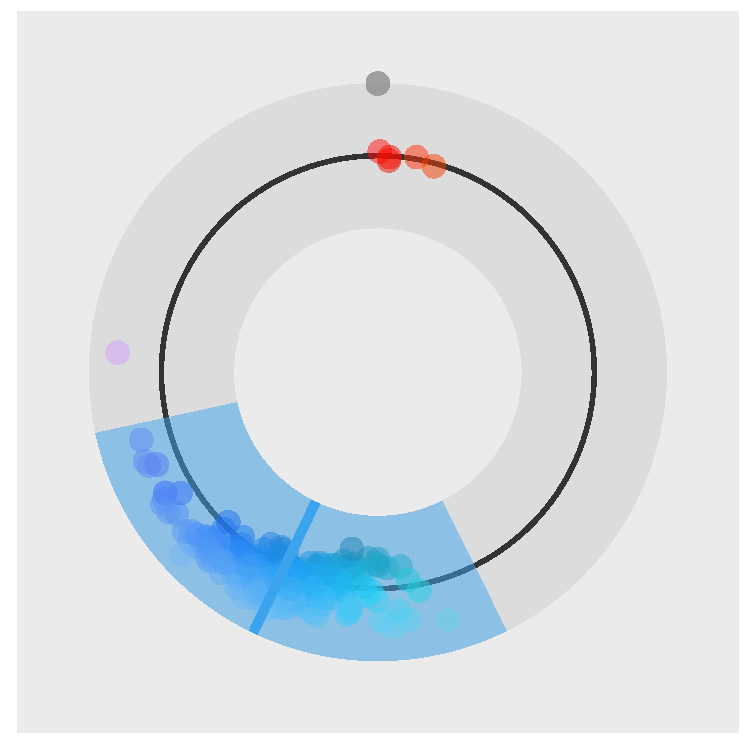
\includegraphics[width=\linewidth]{single_column.pdf}
% 	\caption{\textbf{A random visualization.} This is an example of a figure that spans only across one of the two columns.}
% 	\label{fig:column}
% \end{figure}

% On the other hand, \figurename~\ref{fig:whole} is an example of a figure that spans across the whole page (across both columns) of the report.

% % \begin{figure*} makes the figure take up the entire width of the page
% \begin{figure*}[ht]\centering 
% 	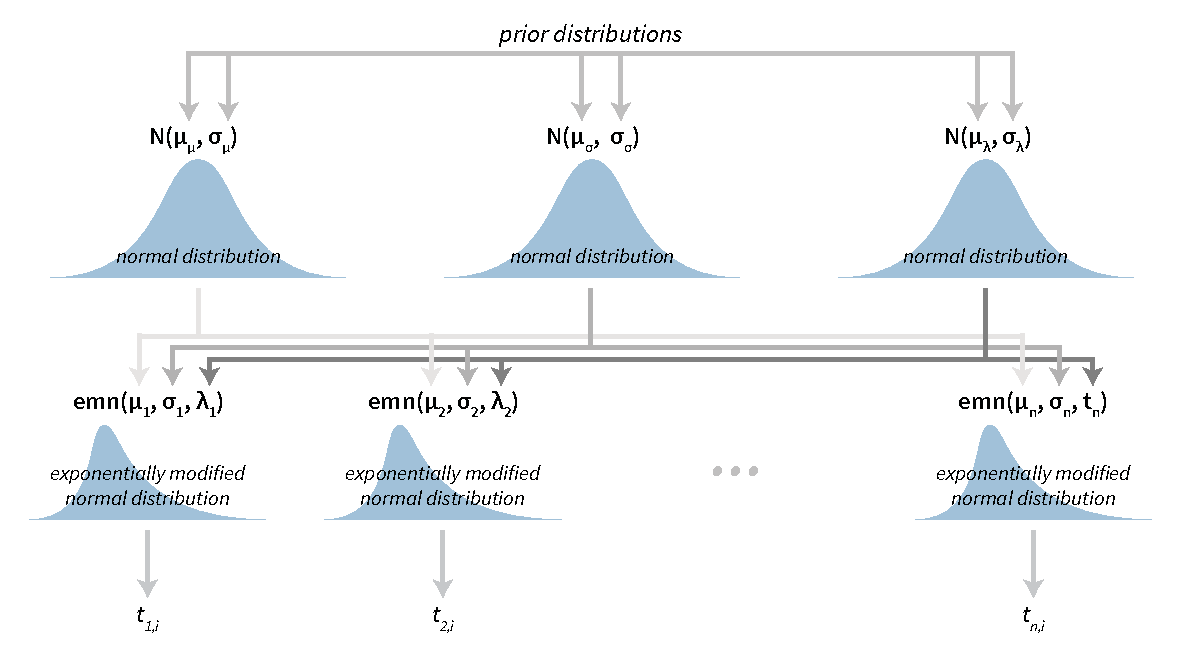
\includegraphics[width=\linewidth]{whole_page.pdf}
% 	\caption{\textbf{Visualization of a Bayesian hierarchical model.} This is an example of a figure that spans the whole width of the report.}
% 	\label{fig:whole}
% \end{figure*}


% \subsection*{Tables}

% Use the table environment to insert tables.

% \begin{table}[hbt]
% 	\caption{Table of grades.}
% 	\centering
% 	\begin{tabular}{l l | r}
% 		\toprule
% 		\multicolumn{2}{c}{Name} \\
% 		\cmidrule(r){1-2}
% 		First name & Last Name & Grade \\
% 		\midrule
% 		John & Doe & $7.5$ \\
% 		Jane & Doe & $10$ \\
% 		Mike & Smith & $8$ \\
% 		\bottomrule
% 	\end{tabular}
% 	\label{tab:label}
% \end{table}


% \subsection*{Code examples}

% You can also insert short code examples. You can specify them manually, or insert a whole file with code. Please avoid inserting long code snippets, advisors will have access to your repositories and can take a look at your code there. If necessary, you can use this technique to insert code (or pseudo code) of short algorithms that are crucial for the understanding of the manuscript.

% \lstset{language=Python}
% \lstset{caption={Insert code directly from a file.}}
% \lstset{label={lst:code_file}}
% \lstinputlisting[language=Python]{code/example.py}

% \lstset{language=R}
% \lstset{caption={Write the code you want to insert.}}
% \lstset{label={lst:code_direct}}
% \begin{lstlisting}
% import(dplyr)
% import(ggplot)

% ggplot(diamonds,
% 	   aes(x=carat, y=price, color=cut)) +
%   geom_point() +
%   geom_smooth()
% \end{lstlisting}

% %------------------------------------------------

% \section*{Results}

% Use the results section to present the final results of your work. Present the results in a objective and scientific fashion. Use visualisations to convey your results in a clear and efficient manner. When comparing results between various techniques use appropriate statistical methodology.

% \subsection*{More random text}

% This text is inserted only to make this template look more like a proper report. Lorem ipsum dolor sit amet, consectetur adipiscing elit. Etiam blandit dictum facilisis. Lorem ipsum dolor sit amet, consectetur adipiscing elit. Interdum et malesuada fames ac ante ipsum primis in faucibus. Etiam convallis tellus velit, quis ornare ipsum aliquam id. Maecenas tempus mauris sit amet libero elementum eleifend. Nulla nunc orci, consectetur non consequat ac, consequat non nisl. Aenean vitae dui nec ex fringilla malesuada. Proin elit libero, faucibus eget neque quis, condimentum laoreet urna. Etiam at nunc quis felis pulvinar dignissim. Phasellus turpis turpis, vestibulum eget imperdiet in, molestie eget neque. Curabitur quis ante sed nunc varius dictum non quis nisl. Donec nec lobortis velit. Ut cursus, libero efficitur dictum imperdiet, odio mi fermentum dui, id vulputate metus velit sit amet risus. Nulla vel volutpat elit. Mauris ex erat, pulvinar ac accumsan sit amet, ultrices sit amet turpis.

% Phasellus in ligula nunc. Vivamus sem lorem, malesuada sed pretium quis, varius convallis lectus. Quisque in risus nec lectus lobortis gravida non a sem. Quisque et vestibulum sem, vel mollis dolor. Nullam ante ex, scelerisque ac efficitur vel, rhoncus quis lectus. Pellentesque scelerisque efficitur purus in faucibus. Maecenas vestibulum vulputate nisl sed vestibulum. Nullam varius turpis in hendrerit posuere.

% Nulla rhoncus tortor eget ipsum commodo lacinia sit amet eu urna. Cras maximus leo mauris, ac congue eros sollicitudin ac. Integer vel erat varius, scelerisque orci eu, tristique purus. Proin id leo quis ante pharetra suscipit et non magna. Morbi in volutpat erat. Vivamus sit amet libero eu lacus pulvinar pharetra sed at felis. Vivamus non nibh a orci viverra rhoncus sit amet ullamcorper sem. Ut nec tempor dui. Aliquam convallis vitae nisi ac volutpat. Nam accumsan, erat eget faucibus commodo, ligula dui cursus nisi, at laoreet odio augue id eros. Curabitur quis tellus eget nunc ornare auctor.


% %------------------------------------------------

% \section*{Discussion}

% Use the Discussion section to objectively evaluate your work, do not just put praise on everything you did, be critical and exposes flaws and weaknesses of your solution. You can also explain what you would do differently if you would be able to start again and what upgrades could be done on the project in the future.


%------------------------------------------------

%\section*{Acknowledgments}

%Special thanks to me myself and I.



%----------------------------------------------------------------------------------------
%	REFERENCE LIST
%----------------------------------------------------------------------------------------
\bibliographystyle{unsrt}
\bibliography{report}


\end{document}